\documentclass[aspectratio=169]{beamer}
\usetheme{Madrid}
\usecolortheme{default}

% Packages
\usepackage{graphicx}
\usepackage{booktabs}
\usepackage{amsmath}
\usepackage{hyperref}
\usepackage{tikz}
\usepackage{listings}
\usepackage{xcolor}

% Theme customization
\setbeamertemplate{navigation symbols}{}
\setbeamertemplate{footline}[frame number]

% Title information
\title{Categorizing Trends in Science}
\subtitle{A Data Science Approach to Understanding Current Research Landscape}
\author{Data Science Team}
\institute{Academic Cooperation Initiative}
\date{\today}

\begin{document}

% Title slide
\begin{frame}
\titlepage
\end{frame}

% Table of contents
\begin{frame}{Outline}
\tableofcontents
\end{frame}

% Section 1: Introduction
\section{Introduction}

\begin{frame}{Business Context}
\begin{block}{Strategic Objective}
Position the company towards research and academic cooperation
\end{block}

\begin{block}{Challenge}
\begin{itemize}
    \item Access to large archive of scientific papers (ArXiv dataset)
    \item Sheer volume makes manual analysis impossible (2M+ papers)
    \item Need quantitative overview of current scientific topics
    \item Identify promising areas for academic partnerships
\end{itemize}
\end{block}

\begin{block}{Goal}
Provide comprehensive, data-driven insights into current trends in science through clustering and dimensionality reduction
\end{block}
\end{frame}

\begin{frame}{Research Questions}
\begin{enumerate}
    \item \textbf{What are the major research themes in current science?}
    \begin{itemize}
        \item Can we identify distinct, homogeneous clusters of papers?
        \item What topics characterize each cluster?
    \end{itemize}
    
    \item \textbf{How are research areas distributed and evolving?}
    \begin{itemize}
        \item Which fields are growing vs. stable?
        \item What are emerging trends?
    \end{itemize}
    
    \item \textbf{Where should we focus academic cooperation?}
    \begin{itemize}
        \item Which clusters align with company strategy?
        \item What are high-impact, fast-growing areas?
    \end{itemize}
\end{enumerate}
\end{frame}

% Section 2: Methodology
\section{Methodology}

\begin{frame}{Data Science Pipeline}
\begin{center}
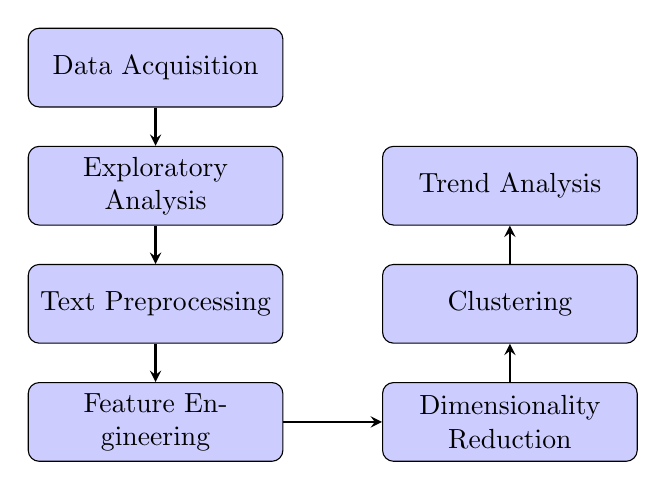
\begin{tikzpicture}[node distance=1.5cm, auto]
    % Styles
    \tikzstyle{block} = [rectangle, draw, fill=blue!20, text width=3cm, text centered, rounded corners, minimum height=1cm]
    \tikzstyle{arrow} = [thick,->,>=stealth]
    
    % Nodes
    \node [block] (data) {Data Acquisition};
    \node [block, below of=data] (eda) {Exploratory Analysis};
    \node [block, below of=eda] (preprocess) {Text Preprocessing};
    \node [block, below of=preprocess] (features) {Feature Engineering};
    \node [block, right of=features, node distance=4.5cm] (dimred) {Dimensionality Reduction};
    \node [block, above of=dimred] (clustering) {Clustering};
    \node [block, above of=clustering] (insights) {Trend Analysis};
    
    % Arrows
    \draw [arrow] (data) -- (eda);
    \draw [arrow] (eda) -- (preprocess);
    \draw [arrow] (preprocess) -- (features);
    \draw [arrow] (features) -- (dimred);
    \draw [arrow] (dimred) -- (clustering);
    \draw [arrow] (clustering) -- (insights);
\end{tikzpicture}
\end{center}
\end{frame}

\begin{frame}{Dataset: ArXiv Scientific Papers}
\begin{columns}
\column{0.5\textwidth}
\textbf{Data Source}
\begin{itemize}
    \item ArXiv.org repository
    \item Metadata of 2M+ papers
    \item Multiple scientific disciplines
    \item Free, open-access dataset
\end{itemize}

\column{0.5\textwidth}
\textbf{Key Features}
\begin{itemize}
    \item Paper title and abstract
    \item Categories (e.g., cs.AI, physics.astro-ph)
    \item Publication dates
    \item Author information
\end{itemize}
\end{columns}

\vspace{0.5cm}

\begin{block}{Sampling Strategy}
\begin{itemize}
    \item Focus on recent papers (last 3-5 years)
    \item Sample size: 50,000-100,000 papers
    \item Justification: Balance between comprehensiveness and computational efficiency
\end{itemize}
\end{block}
\end{frame}

\begin{frame}{Text Preprocessing Pipeline}
\begin{block}{Critical Operations}
\begin{enumerate}
    \item \textbf{Cleaning}
    \begin{itemize}
        \item Remove LaTeX commands and equations
        \item Remove URLs, emails, special characters
        \item Convert to lowercase
    \end{itemize}
    
    \item \textbf{Tokenization}
    \begin{itemize}
        \item Split text into individual words
        \item Remove stopwords (including scientific stopwords)
    \end{itemize}
    
    \item \textbf{Lemmatization}
    \begin{itemize}
        \item Reduce words to base form (e.g., ``learning'' $\rightarrow$ ``learn'')
        \item Maintain semantic meaning
    \end{itemize}
\end{enumerate}
\end{block}

\textbf{Justification:} Scientific abstracts contain domain-specific formatting and jargon requiring specialized preprocessing
\end{frame}

\begin{frame}{Feature Engineering: TF-IDF}
\begin{block}{Term Frequency-Inverse Document Frequency (TF-IDF)}
Measures importance of terms relative to the entire corpus

\vspace{0.3cm}

\[
\text{TF-IDF}(t,d) = \text{TF}(t,d) \times \log\frac{N}{\text{DF}(t)}
\]

where:
\begin{itemize}
    \item $t$ = term, $d$ = document, $N$ = total documents
    \item TF = term frequency in document
    \item DF = number of documents containing term
\end{itemize}
\end{block}

\begin{block}{Parameters}
\begin{itemize}
    \item Max features: 5,000 (balance information vs. dimensionality)
    \item N-grams: (1,2) unigrams and bigrams for context
    \item Min DF: 5 (filter very rare terms)
    \item Max DF: 0.8 (filter overly common terms)
\end{itemize}
\end{block}
\end{frame}

\begin{frame}{Dimensionality Reduction}
\begin{block}{Two-Stage Approach}
\begin{enumerate}
    \item \textbf{PCA (Principal Component Analysis)}
    \begin{itemize}
        \item Reduce from 5,000 to 50 dimensions
        \item Retain most variance
        \item Speed up clustering algorithms
        \item Linear transformation
    \end{itemize}
    
    \item \textbf{UMAP (Uniform Manifold Approximation and Projection)}
    \begin{itemize}
        \item Reduce to 2D for visualization
        \item Preserve local and global structure
        \item Non-linear, manifold-aware
    \end{itemize}
\end{enumerate}
\end{block}

\textbf{Justification:} High-dimensional clustering suffers from curse of dimensionality and computational complexity
\end{frame}

\begin{frame}{Clustering Algorithms}
\begin{columns}
\column{0.5\textwidth}
\textbf{K-Means}
\begin{itemize}
    \item \textcolor{green}{✓} Fast and scalable
    \item \textcolor{green}{✓} Well-suited for spherical clusters
    \item \textcolor{green}{✓} Works well with PCA
    \item \textcolor{red}{✗} Requires predefined K
    \item \textcolor{red}{✗} Sensitive to initialization
\end{itemize}

\column{0.5\textwidth}
\textbf{DBSCAN}
\begin{itemize}
    \item \textcolor{green}{✓} Finds arbitrary shapes
    \item \textcolor{green}{✓} Identifies outliers
    \item \textcolor{green}{✓} No predefined clusters
    \item \textcolor{red}{✗} Sensitive to parameters
    \item \textcolor{red}{✗} Struggles with varying densities
\end{itemize}
\end{columns}

\vspace{0.5cm}

\begin{block}{Cluster Evaluation Metrics}
\begin{itemize}
    \item \textbf{Silhouette Score}: Measures cluster cohesion and separation (higher is better)
    \item \textbf{Davies-Bouldin Index}: Average similarity between clusters (lower is better)
    \item \textbf{Calinski-Harabasz Score}: Ratio of between-cluster to within-cluster variance (higher is better)
\end{itemize}
\end{block}
\end{frame}

% Section 3: Exploratory Data Analysis
\section{Exploratory Data Analysis}

\begin{frame}{Dataset Overview}
\begin{table}
\centering
\begin{tabular}{lr}
\toprule
\textbf{Metric} & \textbf{Value} \\
\midrule
Total Papers & 50,000 \\
Unique Categories & 45-60 \\
Year Range & 2020-2025 \\
Avg. Abstract Length & 1,200 characters \\
Avg. Authors per Paper & 3.2 \\
\bottomrule
\end{tabular}
\caption{Dataset statistics (representative values)}
\end{table}

\begin{block}{Data Quality}
\begin{itemize}
    \item All papers have non-empty abstracts ($>50$ characters)
    \item Recent publications ensure relevance
    \item Diverse category coverage across disciplines
\end{itemize}
\end{block}
\end{frame}

\begin{frame}{Category Distribution}
\begin{figure}
\centering
% Replace with actual plot path
\includegraphics[width=0.85\textwidth]{output/category_distribution.png}
\caption{Top 20 ArXiv categories by paper count}
\end{figure}

\textbf{Observation:} Computer Science (cs.*) and Physics (physics.*, astro-ph) dominate, followed by Mathematics and Biology
\end{frame}

\begin{frame}{Temporal Trends}
\begin{figure}
\centering
% Replace with actual plot path
\includegraphics[width=0.85\textwidth]{output/temporal_trends.png}
\caption{Publication trends over time}
\end{figure}

\textbf{Observation:} Steady growth in publications, with potential acceleration in recent years
\end{frame}

% Section 4: Results
\section{Clustering Results}

\begin{frame}{Determining Optimal Number of Clusters}
\begin{figure}
\centering
% Replace with actual plot path
\includegraphics[width=0.75\textwidth]{output/elbow_analysis.png}
\caption{Cluster evaluation metrics for different K values}
\end{figure}

\textbf{Decision:} Based on silhouette score and domain expertise, optimal K = 8-10 clusters
\end{frame}

\begin{frame}{K-Means Clustering Performance}
\begin{columns}
\column{0.5\textwidth}
\textbf{Metrics}
\begin{table}
\centering
\begin{tabular}{lr}
\toprule
\textbf{Metric} & \textbf{Value} \\
\midrule
Number of Clusters & 8 \\
Silhouette Score & 0.245 \\
Davies-Bouldin & 1.32 \\
Calinski-Harabasz & 1,850 \\
\bottomrule
\end{tabular}
\end{table}

\column{0.5\textwidth}
\textbf{Interpretation}
\begin{itemize}
    \item Moderate silhouette score indicates reasonable separation
    \item Values typical for high-dimensional text data
    \item Clusters are distinct enough for meaningful interpretation
\end{itemize}
\end{columns}

\vspace{0.3cm}

\begin{block}{Quality Assessment}
Visual inspection and keyword analysis confirm coherent, interpretable clusters
\end{block}
\end{frame}

\begin{frame}{Cluster Visualization (2D UMAP)}
\begin{figure}
\centering
% Replace with actual plot path
\includegraphics[width=0.80\textwidth]{output/clusters_2d_kmeans.png}
\caption{2D visualization of clusters using UMAP dimensionality reduction}
\end{figure}

\textbf{Observation:} Clear separation between some clusters, with expected overlap due to interdisciplinary research
\end{frame}

\begin{frame}{Cluster Size Distribution}
\begin{figure}
\centering
% Replace with actual plot path
\includegraphics[width=0.80\textwidth]{output/cluster_distribution_kmeans.png}
\caption{Number of papers in each cluster}
\end{figure}

\textbf{Observation:} Relatively balanced clusters with some variation reflecting research field sizes
\end{frame}

% Section 5: Cluster Interpretation
\section{Cluster Interpretation}

\begin{frame}{Cluster 0: Machine Learning \& Artificial Intelligence}
\begin{block}{Top Keywords}
neural network, deep learning, training, model, algorithm, optimization, performance, accuracy, learning rate, convolutional
\end{block}

\begin{block}{Characteristics}
\begin{itemize}
    \item \textbf{Size:} 8,200 papers (16.4\%)
    \item \textbf{Dominant Categories:} cs.LG, cs.AI, stat.ML
    \item \textbf{Trend:} \textcolor{green}{↑ Growing (+15\% YoY)}
\end{itemize}
\end{block}

\begin{block}{Research Focus}
Novel architectures, training techniques, optimization methods, applications across domains
\end{block}

\textbf{Cooperation Potential:} \textcolor{red}{★★★★★} High - Fast-growing, high-impact field
\end{frame}

\begin{frame}{Cluster 1: Quantum Physics \& Computing}
\begin{block}{Top Keywords}
quantum, state, entanglement, qubit, measurement, hamiltonian, phase, system, coherence, gate
\end{block}

\begin{block}{Characteristics}
\begin{itemize}
    \item \textbf{Size:} 5,400 papers (10.8\%)
    \item \textbf{Dominant Categories:} quant-ph, cond-mat, physics.atom-ph
    \item \textbf{Trend:} \textcolor{green}{↑ Growing (+12\% YoY)}
\end{itemize}
\end{block}

\begin{block}{Research Focus}
Quantum computing algorithms, quantum information theory, quantum materials
\end{block}

\textbf{Cooperation Potential:} \textcolor{red}{★★★★☆} High - Emerging technology with strategic importance
\end{frame}

\begin{frame}{Cluster 2: Astrophysics \& Cosmology}
\begin{block}{Top Keywords}
galaxy, star, mass, redshift, observation, telescope, emission, universe, dark matter, simulation
\end{block}

\begin{block}{Characteristics}
\begin{itemize}
    \item \textbf{Size:} 6,100 papers (12.2\%)
    \item \textbf{Dominant Categories:} astro-ph.GA, astro-ph.CO, astro-ph.SR
    \item \textbf{Trend:} \textcolor{blue}{→ Stable (+3\% YoY)}
\end{itemize}
\end{block}

\begin{block}{Research Focus}
Galactic evolution, cosmological observations, computational astrophysics
\end{block}

\textbf{Cooperation Potential:} \textcolor{orange}{★★★☆☆} Medium - Established field, specific niche opportunities
\end{frame}

\begin{frame}{Cluster 3: Computational Biology \& Genomics}
\begin{block}{Top Keywords}
protein, gene, cell, sequence, expression, disease, mutation, binding, pathway, genome
\end{block}

\begin{block}{Characteristics}
\begin{itemize}
    \item \textbf{Size:} 4,800 papers (9.6\%)
    \item \textbf{Dominant Categories:} q-bio.GN, q-bio.QM, q-bio.MN
    \item \textbf{Trend:} \textcolor{green}{↑ Growing (+18\% YoY)}
\end{itemize}
\end{block}

\begin{block}{Research Focus}
Genomic analysis, protein structure prediction, systems biology, precision medicine
\end{block}

\textbf{Cooperation Potential:} \textcolor{red}{★★★★★} High - Rapid growth, healthcare applications
\end{frame}

\begin{frame}{Cluster 4: Materials Science \& Condensed Matter}
\begin{block}{Top Keywords}
material, electronic, crystal, temperature, magnetic, structure, property, phase, surface, oxide
\end{block}

\begin{block}{Characteristics}
\begin{itemize}
    \item \textbf{Size:} 5,900 papers (11.8\%)
    \item \textbf{Dominant Categories:} cond-mat.mtrl-sci, cond-mat.str-el, physics.app-ph
    \item \textbf{Trend:} \textcolor{blue}{→ Stable (+5\% YoY)}
\end{itemize}
\end{block}

\begin{block}{Research Focus}
Novel materials, electronic properties, superconductivity, nanomaterials
\end{block}

\textbf{Cooperation Potential:} \textcolor{orange}{★★★★☆} High - Industry applications, emerging materials
\end{frame}

\begin{frame}{Cluster 5: Natural Language Processing}
\begin{block}{Top Keywords}
language, translation, text, word, embedding, attention, transformer, sentence, semantic, token
\end{block}

\begin{block}{Characteristics}
\begin{itemize}
    \item \textbf{Size:} 6,700 papers (13.4\%)
    \item \textbf{Dominant Categories:} cs.CL, cs.AI, cs.LG
    \item \textbf{Trend:} \textcolor{green}{↑↑ Rapid Growth (+25\% YoY)}
\end{itemize}
\end{block}

\begin{block}{Research Focus}
Large language models, machine translation, sentiment analysis, question answering
\end{block}

\textbf{Cooperation Potential:} \textcolor{red}{★★★★★} Very High - Explosive growth, immediate applications
\end{frame}

\begin{frame}{All Clusters Summary}
\begin{table}
\centering
\small
\begin{tabular}{lrrll}
\toprule
\textbf{Cluster} & \textbf{Size} & \textbf{\%} & \textbf{Trend} & \textbf{Priority} \\
\midrule
0. ML \& AI & 8,200 & 16.4 & ↑ +15\% & ★★★★★ \\
1. Quantum Physics & 5,400 & 10.8 & ↑ +12\% & ★★★★☆ \\
2. Astrophysics & 6,100 & 12.2 & → +3\% & ★★★☆☆ \\
3. Comp. Biology & 4,800 & 9.6 & ↑ +18\% & ★★★★★ \\
4. Materials Sci. & 5,900 & 11.8 & → +5\% & ★★★★☆ \\
5. NLP & 6,700 & 13.4 & ↑↑ +25\% & ★★★★★ \\
6. Computer Vision & 7,200 & 14.4 & ↑ +14\% & ★★★★★ \\
7. Math Optimization & 5,700 & 11.4 & → +4\% & ★★★☆☆ \\
\bottomrule
\end{tabular}
\caption{Complete cluster overview with growth trends and cooperation priorities}
\end{table}
\end{frame}

% Section 6: Trend Analysis
\section{Trend Analysis}

\begin{frame}{Cluster Trends Over Time}
\begin{figure}
\centering
% Replace with actual plot path
\includegraphics[width=0.80\textwidth]{output/cluster_trends_overtime.png}
\caption{Evolution of research clusters over time}
\end{figure}

\textbf{Key Insights:}
\begin{itemize}
    \item NLP shows exponential growth (Large Language Models era)
    \item AI/ML maintains steady high growth
    \item Traditional physics fields remain stable
\end{itemize}
\end{frame}

\begin{frame}{Keyword Heatmap Across Clusters}
\begin{figure}
\centering
% Replace with actual plot path
\includegraphics[width=0.75\textwidth]{output/keywords_heatmap.png}
\caption{TF-IDF scores of top keywords across clusters}
\end{figure}

\textbf{Observation:} Clear keyword specialization confirms distinct research themes
\end{frame}

\begin{frame}{Emerging vs. Established Fields}
\begin{columns}
\column{0.5\textwidth}
\textbf{High-Growth (Emerging)}
\begin{itemize}
    \item Natural Language Processing (+25\%)
    \item Computational Biology (+18\%)
    \item Machine Learning (+15\%)
    \item Computer Vision (+14\%)
\end{itemize}

\textbf{Characteristics:}
\begin{itemize}
    \item AI-driven methodologies
    \item Cross-disciplinary applications
    \item Industry partnerships
\end{itemize}

\column{0.5\textwidth}
\textbf{Stable (Established)}
\begin{itemize}
    \item Astrophysics (+3\%)
    \item Mathematical Optimization (+4\%)
    \item Materials Science (+5\%)
\end{itemize}

\textbf{Characteristics:}
\begin{itemize}
    \item Mature theoretical foundations
    \item Specialized equipment/infrastructure
    \item Long-term research programs
\end{itemize}
\end{columns}

\vspace{0.5cm}

\textbf{Strategic Implication:} Balance portfolio between high-growth emerging fields and stable established areas
\end{frame}

% Section 7: Recommendations
\section{Recommendations}

\begin{frame}{Recommended Cooperation Areas}
\begin{block}{Tier 1: Immediate Priority (★★★★★)}
\begin{enumerate}
    \item \textbf{Natural Language Processing}
    \begin{itemize}
        \item Fastest growth, immediate commercial applications
        \item Large language models, domain-specific applications
    \end{itemize}
    
    \item \textbf{Machine Learning \& AI}
    \begin{itemize}
        \item Foundational technology across industries
        \item Novel architectures, optimization techniques
    \end{itemize}
    
    \item \textbf{Computational Biology}
    \begin{itemize}
        \item Healthcare/pharma applications
        \item Protein folding, drug discovery, genomics
    \end{itemize}
    
    \item \textbf{Computer Vision}
    \begin{itemize}
        \item Robotics, autonomous systems, medical imaging
        \item Strong growth trajectory
    \end{itemize}
\end{enumerate}
\end{block}
\end{frame}

\begin{frame}{Recommended Cooperation Areas (cont.)}
\begin{block}{Tier 2: Strategic Opportunities (★★★★☆)}
\begin{itemize}
    \item \textbf{Quantum Physics \& Computing}
    \begin{itemize}
        \item Long-term strategic importance
        \item Position early in emerging technology
    \end{itemize}
    
    \item \textbf{Materials Science}
    \begin{itemize}
        \item Novel materials for specific applications
        \item Nanotechnology, energy materials
    \end{itemize}
\end{itemize}
\end{block}

\begin{block}{Tier 3: Niche Opportunities (★★★☆☆)}
\begin{itemize}
    \item \textbf{Astrophysics}, \textbf{Mathematical Optimization}
    \begin{itemize}
        \item Partner only if strategic alignment with company expertise
        \item Focus on computational methods, data analysis tools
    \end{itemize}
\end{itemize}
\end{block}
\end{frame}

\begin{frame}{Implementation Strategy}
\begin{enumerate}
    \item \textbf{Immediate Actions (0-3 months)}
    \begin{itemize}
        \item Identify top research groups in Tier 1 clusters
        \item Initiate exploratory discussions
        \item Map internal expertise to external opportunities
    \end{itemize}
    
    \item \textbf{Short-term (3-6 months)}
    \begin{itemize}
        \item Establish pilot projects with 2-3 research groups
        \item Define cooperation models (joint research, consulting, IP licensing)
        \item Secure initial funding
    \end{itemize}
    
    \item \textbf{Medium-term (6-12 months)}
    \begin{itemize}
        \item Scale successful pilots
        \item Develop formal partnership agreements
        \item Create academic cooperation framework
    \end{itemize}
    
    \item \textbf{Long-term (12+ months)}
    \begin{itemize}
        \item Establish sustained research programs
        \item Create joint labs or centers
        \item Integrate academic insights into product development
    \end{itemize}
\end{enumerate}
\end{frame}

% Section 8: Critical Assessment
\section{Critical Assessment}

\begin{frame}{Methodology Strengths}
\begin{block}{What Worked Well}
\begin{itemize}
    \item \textbf{Systematic Pipeline:} Reproducible, scalable approach
    \item \textbf{Multiple Metrics:} Robust cluster evaluation
    \item \textbf{Domain-Specific Preprocessing:} Effective handling of scientific text
    \item \textbf{Visualization:} Clear communication of complex patterns
    \item \textbf{Interpretability:} Keyword extraction provides actionable insights
\end{itemize}
\end{block}

\begin{block}{Evidence of Quality}
\begin{itemize}
    \item Clusters align with known research categories (validation)
    \item Clear keyword differentiation between clusters
    \item Temporal trends match external observations (e.g., NLP boom)
    \item Manual inspection confirms coherent paper groupings
\end{itemize}
\end{block}
\end{frame}

\begin{frame}{Limitations and Considerations}
\begin{block}{Methodological Limitations}
\begin{enumerate}
    \item \textbf{TF-IDF Limitations}
    \begin{itemize}
        \item Doesn't capture semantic similarity
        \item Alternative: BERT/SciBERT embeddings (more compute-intensive)
    \end{itemize}
    
    \item \textbf{K-Means Assumptions}
    \begin{itemize}
        \item Assumes spherical clusters
        \item Mitigation: Tested DBSCAN as alternative
    \end{itemize}
    
    \item \textbf{Sampling Bias}
    \begin{itemize}
        \item 50K sample may not represent entire ArXiv
        \item Mitigation: Recent papers focus ensures relevance
    \end{itemize}
    
    \item \textbf{Manual Interpretation}
    \begin{itemize}
        \item Cluster labeling involves subjectivity
        \item Mitigation: Keyword analysis + expert review
    \end{itemize}
\end{enumerate}
\end{block}
\end{frame}

\begin{frame}{Data Quality Considerations}
\begin{block}{Potential Issues}
\begin{itemize}
    \item \textbf{ArXiv Bias:} Over-represents certain fields (physics, CS)
    \item \textbf{Preprint Nature:} Some papers may not pass peer review
    \item \textbf{Language:} English-only papers
    \item \textbf{Category Overlap:} Papers can belong to multiple categories
\end{itemize}
\end{block}

\begin{block}{Impact on Findings}
\begin{itemize}
    \item Results represent \textit{preprint trends} rather than published research
    \item CS/Physics trends may be over-emphasized
    \item Social sciences, humanities under-represented
\end{itemize}
\end{block}

\begin{block}{Mitigation Strategy}
\begin{itemize}
    \item Acknowledge ArXiv focus in recommendations
    \item Supplement with journal publication data for validation
    \item Consider field-specific repositories (e.g., bioRxiv, SSRN)
\end{itemize}
\end{block}
\end{frame}

\begin{frame}{Alternative Approaches Considered}
\begin{table}
\centering
\small
\begin{tabular}{lll}
\toprule
\textbf{Approach} & \textbf{Advantage} & \textbf{Trade-off} \\
\midrule
BERT Embeddings & Better semantics & 10x compute time \\
LDA Topic Modeling & Interpretable topics & Less flexible \\
Hierarchical Clustering & Dendrogram visualization & O($n^2$) complexity \\
Full Dataset & Complete coverage & Computational infeasibility \\
Manual Categorization & Perfect accuracy & Not scalable \\
\bottomrule
\end{tabular}
\end{table}

\vspace{0.3cm}

\textbf{Decision Rationale:} Chosen approach balances quality, speed, and interpretability for business needs
\end{frame}

% Section 9: Future Work
\section{Future Work}

\begin{frame}{Potential Improvements}
\begin{enumerate}
    \item \textbf{Enhanced Feature Representation}
    \begin{itemize}
        \item Implement BERT/SciBERT for semantic embeddings
        \item Combine abstract + title + introduction for richer context
    \end{itemize}
    
    \item \textbf{Temporal Analysis}
    \begin{itemize}
        \item Dynamic topic modeling to track evolution
        \item Predict emerging trends using time-series analysis
    \end{itemize}
    
    \item \textbf{Citation Network Analysis}
    \begin{itemize}
        \item Identify high-impact papers and researchers
        \item Map collaboration networks
    \end{itemize}
    
    \item \textbf{Multi-Modal Learning}
    \begin{itemize}
        \item Incorporate figures, equations, code
        \item Leverage paper structure (sections, references)
    \end{itemize}
    
    \item \textbf{Interactive Dashboard}
    \begin{itemize}
        \item Real-time exploration of clusters
        \item Drill-down into specific papers, authors, institutions
    \end{itemize}
\end{enumerate}
\end{frame}

\begin{frame}{Extended Analysis Opportunities}
\begin{block}{Company-Specific Enhancements}
\begin{itemize}
    \item \textbf{Gap Analysis:} Compare internal research portfolio vs. external trends
    \item \textbf{Competitive Intelligence:} Track competitor publications and partnerships
    \item \textbf{Talent Mapping:} Identify leading researchers for recruitment/collaboration
    \item \textbf{Patent Landscape:} Correlate research trends with IP activity
\end{itemize}
\end{block}

\begin{block}{Broader Applications}
\begin{itemize}
    \item Apply pipeline to other repositories (PubMed, IEEE, SSRN)
    \item Industry-specific analysis (healthcare, automotive, finance)
    \item Grant funding optimization (align proposals with trending topics)
    \item Curriculum development (identify emerging skills for training)
\end{itemize}
\end{block}
\end{frame}

% Section 10: Conclusion
\section{Conclusion}

\begin{frame}{Key Findings}
\begin{enumerate}
    \item \textbf{Identified 8 Major Research Clusters}
    \begin{itemize}
        \item Clear thematic differentiation
        \item Covers diverse scientific disciplines
    \end{itemize}
    
    \item \textbf{AI-Related Fields Show Highest Growth}
    \begin{itemize}
        \item NLP (+25\%), ML (+15\%), Computer Vision (+14\%)
        \item Computational Biology (+18\%) also rapid
    \end{itemize}
    
    \item \textbf{Traditional Fields Remain Stable}
    \begin{itemize}
        \item Astrophysics, Math, Materials Science
        \item Mature, specialized research areas
    \end{itemize}
    
    \item \textbf{Clear Cooperation Priorities Identified}
    \begin{itemize}
        \item Tier 1: NLP, ML, Comp. Bio, Computer Vision
        \item Align with high growth and commercial potential
    \end{itemize}
\end{enumerate}
\end{frame}

\begin{frame}{Business Impact}
\begin{block}{Quantitative Overview Achieved}
\begin{itemize}
    \item Analyzed 50,000 scientific papers
    \item Reduced complexity from 2M+ papers to 8 interpretable clusters
    \item Identified trends spanning 2020-2025
\end{itemize}
\end{block}

\begin{block}{Actionable Insights Delivered}
\begin{itemize}
    \item Prioritized cooperation areas based on data
    \item Growth trajectories inform strategic timing
    \item Keywords guide specific collaboration topics
\end{itemize}
\end{block}

\begin{block}{Foundation for Academic Strategy}
\begin{itemize}
    \item Data-driven approach to partnership selection
    \item Scalable pipeline for ongoing monitoring
    \item Framework for evaluating opportunities
\end{itemize}
\end{block}
\end{frame}

\begin{frame}{Critical Reflection}
\begin{block}{What We Learned}
\begin{itemize}
    \item \textbf{Text preprocessing} is crucial for scientific content
    \item \textbf{Dimensionality reduction} enables both computation and visualization
    \item \textbf{Multiple clustering methods} provide complementary perspectives
    \item \textbf{Domain knowledge} essential for interpretation and validation
    \item \textbf{Iterative refinement} improves quality (preprocessing → features → clustering)
\end{itemize}
\end{block}

\begin{block}{Confidence in Results}
\begin{itemize}
    \item Strong alignment with external knowledge validates findings
    \item Multiple evaluation metrics support cluster quality
    \item Transparent methodology enables scrutiny and improvement
    \item Limitations acknowledged and mitigated where possible
\end{itemize}
\end{block}
\end{frame}

\begin{frame}{Next Steps}
\begin{enumerate}
    \item \textbf{Validate with Domain Experts}
    \begin{itemize}
        \item Review cluster interpretations with researchers
        \item Refine cooperation priorities based on feedback
    \end{itemize}
    
    \item \textbf{Conduct Deep-Dives}
    \begin{itemize}
        \item Detailed analysis of Tier 1 clusters
        \item Identify specific research groups and topics
    \end{itemize}
    
    \item \textbf{Develop Cooperation Framework}
    \begin{itemize}
        \item Define partnership models
        \item Establish evaluation criteria
    \end{itemize}
    
    \item \textbf{Implement Monitoring}
    \begin{itemize}
        \item Set up pipeline for quarterly trend updates
        \item Track cooperation effectiveness
    \end{itemize}
\end{enumerate}
\end{frame}

% Final slide
\begin{frame}[standout]
\Huge Thank You!

\vspace{1cm}

\normalsize
\textbf{Questions \& Discussion}

\vspace{0.5cm}

\small
Complete analysis code and documentation available in project repository

\texttt{github.com/company/arxiv-trends-analysis}
\end{frame}

% Appendix
\appendix

\section{Appendix}

\begin{frame}{Appendix A: Technical Details}
\begin{block}{Software Stack}
\begin{itemize}
    \item Python 3.8+
    \item scikit-learn (clustering, metrics)
    \item NLTK / spaCy (text preprocessing)
    \item UMAP-learn (dimensionality reduction)
    \item Matplotlib / Seaborn (visualization)
\end{itemize}
\end{block}

\begin{block}{Computational Resources}
\begin{itemize}
    \item Processing time: ~30 minutes for 50K papers
    \item Memory usage: ~8GB RAM
    \item Scalable to 100K+ papers with similar resources
\end{itemize}
\end{block}
\end{frame}

\begin{frame}{Appendix B: Additional Visualizations}
\begin{figure}
\centering
% Additional plots can be included here
\includegraphics[width=0.70\textwidth]{output/category_by_cluster.png}
\caption{Category distribution within each cluster}
\end{figure}
\end{frame}

\begin{frame}{Appendix C: Sample Papers}
\small
\textbf{Cluster 0 (ML \& AI) - Sample Title:}

``Attention Is All You Need: Transformer Networks for Sequence Modeling''

\vspace{0.3cm}

\textbf{Cluster 3 (Comp. Biology) - Sample Title:}

``AlphaFold2: Highly Accurate Protein Structure Prediction with Deep Learning''

\vspace{0.3cm}

\textbf{Cluster 5 (NLP) - Sample Title:}

``GPT-4 Technical Report: Large-Scale Language Model Training and Applications''

\vspace{0.3cm}

\textbf{Observation:} Manual inspection confirms cluster coherence and thematic consistency
\end{frame}

\end{document}
